\section{Quantification}

As mentioned in \cref{sec:crna_quantification}, all the \gls{bsj} detection
tools also quantify the number of reads supporting each \gls{bsj}.
However, there are several tools that focus on the quantification of
\gls{crna}s based on previously detected \gls{bsj}s.
nf-core/circrna offers two such tools: CIRIquant and psirc-quant.

Due to the lack of a ground truth or a gold standard, the quantification
results were compared to each other.
The correlation heatmaps in \cref{fig:correlation_heatmap} show the Pearson
correlation coefficient between the quantification results of the detection
tools, multiple aggregations of the detection tools, and the quantification
tools.

\begin{figure}[ht]
    \begin{tabular}{cc}
        \begin{subfigure}{0.5\textwidth}
            \centering

            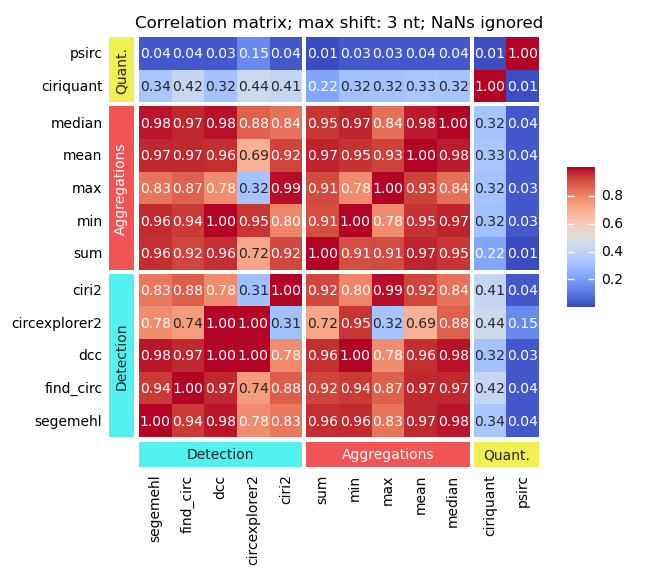
\includegraphics[width=\linewidth]{chapters/4_results_and_discussion/figures/quantification/correlation_heatmap_3_na.png}
            \caption{Missing values treated as NaN}
            \label{fig:correlation_heatmap_3_na}
        \end{subfigure}
         &
        \begin{subfigure}{0.5\textwidth}
            \centering

            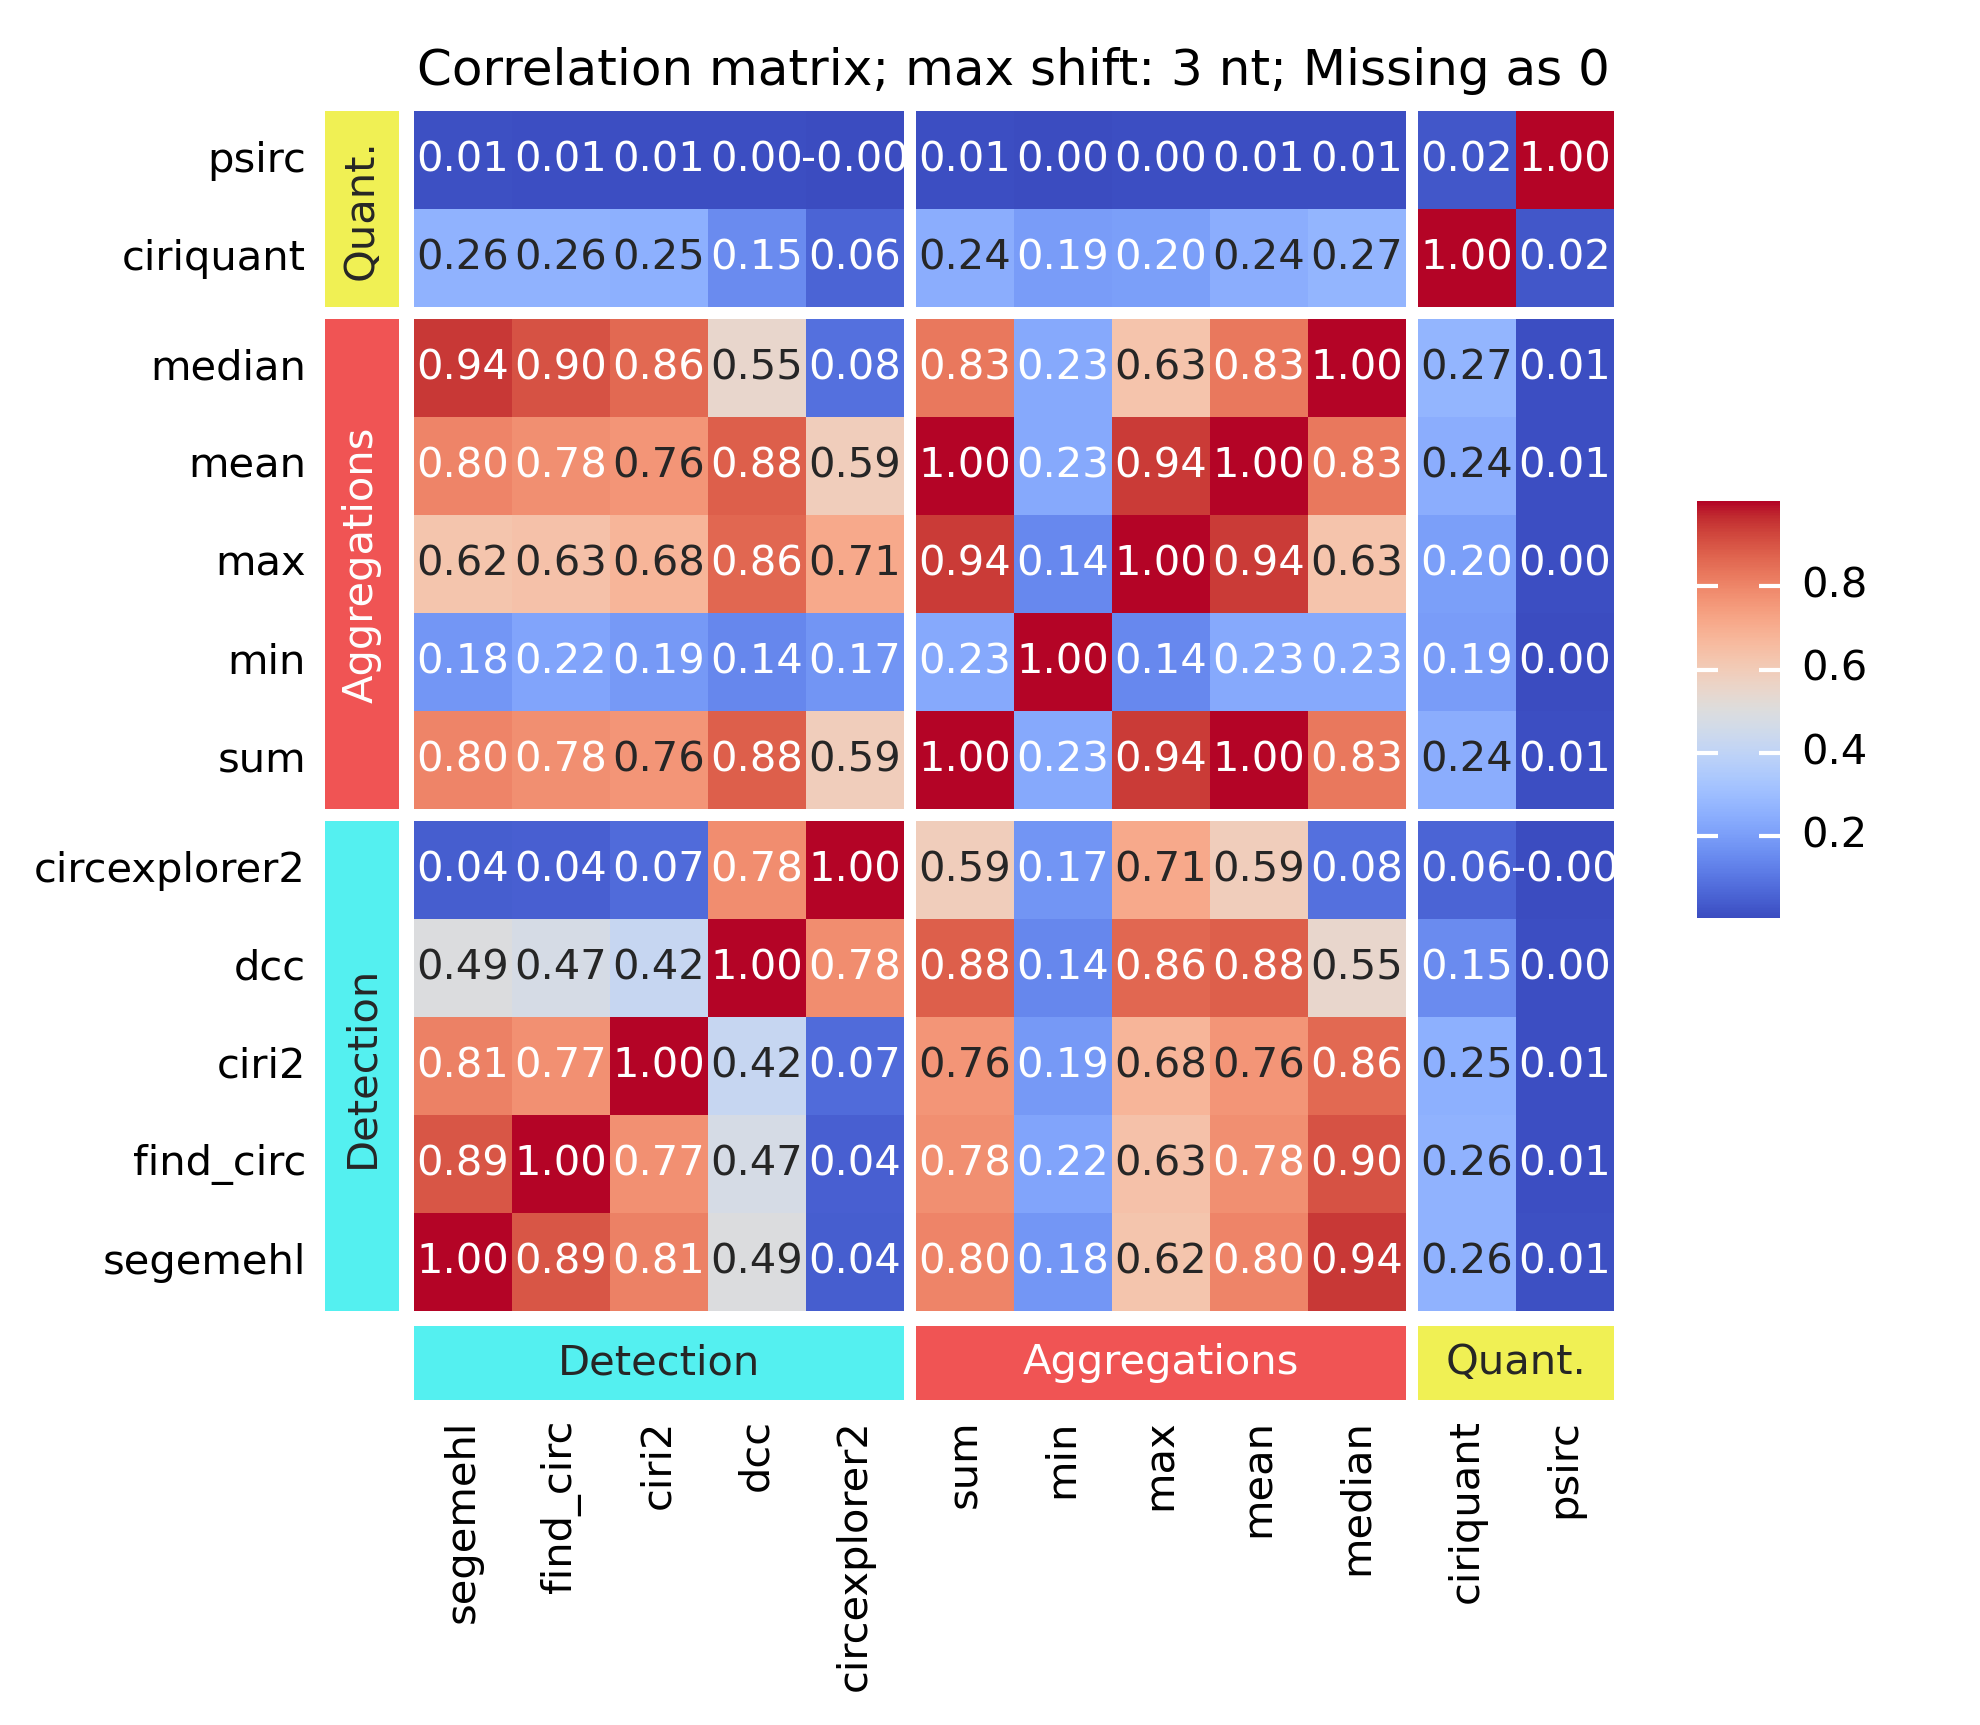
\includegraphics[width=\linewidth]{chapters/4_results_and_discussion/figures/quantification/correlation_heatmap_3_0.png}
            \caption{Missing values treated as 0}
            \label{fig:correlation_heatmap_3_0}
        \end{subfigure}
    \end{tabular}
    \caption{Pearson correlation heatmap between the quantification results of
        the detection tools, multiple aggregations of the detection tools, and
        the quantification tools.
        The expression values were scaled so that the sum per sample and tool was
        constant.
        For each detected \gls{bsj}, expression information of all \gls{bsj}s within a
        \textit{max shift} of 3 was summed.
        While treating missing values as NaN results in higher correlations overall,
        treating the zeros as actual 0 values better reflects the underlying data.
        This is because missing values mean that a tool did not detect any reads
        supporting a \gls{bsj} (thus not outputting anything), which is equal to the
        definition of 0 expression.
        In \cref{fig:correlation_heatmap_3_0}, we can see that the quantification tools
        show relatively low correlation with the detection tools and aggregations.
    } \label{fig:correlation_heatmap} \end{figure}

\subsection{Quantification tools}
Interestingly, the quantification tools show relatively low correlation with
the detection tools and aggregations.
While both show robust results in their respective publications, they were only
tested on paired end data\supercite{zhang_accurate_2020,yu_quantifying_2021}.

\paragraph{psirc}
For psirc, there is an additional complication: As mentioned in
\cref{sec:psirc}, it expects the full-length isoform \gls{crna}sequence as
input.
As we only have single-end data, we cannot provide this information.
Therefor, the entire sequence within the \gls{bsj} boundaries is used as the
\gls{crna} sequence.
While psirc uses the information that the sequence is circular when
constructing the Transcript de Bruijn Graph (T-DBG), it does not treat reads
spanning the \gls{bsj} differently from reads that do
not\supercite{yu_quantifying_2021}.

While due to the lack of ground truth it is impossible to say that the
quantification results of psirc are wrong, the low correlation with the
detection tools indicates that they are at least questionable in this context.
Thus, I will not use the quantification results of psirc in the following
analyses.

\paragraph{CIRIquant}
CIRIquant, on the other hand, shows a higher correlation with the detection
tools and aggregations.
However, it is still relatively low ($<$0.3 in all comparisons when treating
missing values as 0).
Here, it is not clear why the correlation is so low, as CIRIquant uses a
similar approach to the detection tools.
Again, the lack of a ground truth makes it impossible to say whether the
quantification results of CIRIquant are trustworthy in this setting.

\subsection{Detection tools}
It appears like there are two groups of detection tools: One including
Segemehl, find\_circ and ciri2, and the other including DCC and CircExplorer2.
Both show high internal correlation in both settings ($>$0.75) and low
correlation between the groups ($\leq$0.5 for missing values treated as 0).

%TODO: Add reasoning

\subsection{Aggregations}
Many of the investigated aggregations seem to be able to smoothen out the
differences between the two groups of detection tools.
In the following paragraphs, I will look into the individual aggregations in
more detail.

\paragraph{min}
Using the minimum expression value of all tools for each \gls{bsj}
interestingly results in high correlations with find\_circ and Segemehl wenn
treating missing values as NaN.
In this setting, the minimum expression will be the smallest value of tools
with an expression value.
When looking at the behaviour of the min aggregation when treating missing
values as 0, we see that all correlation values are $<$0.25.
Here, the min aggregation will be 0 if any of the tools did not detect any
reads supporting a \gls{bsj}, which is true for many \gls{bsj}s.

\paragraph{max}
The max aggregation interestingly has high correlations with DCC and
CircExplorer2 in the NaN setting.
This indicates that - if they detect a \gls{bsj} - they often detect a high
number of reads supporting it.
In the 0 setting, the max aggregation achieved a correlation $>$0.6 with all
tools, thus yielding stable, but slightly worse results than the following
aggregations.

\paragraph{sum}
The sum aggregation results in robust correlations in both settings.
While the correlation with CircExplorer2 is lower than with the other tools in
the 0 setting, this is mostly due to the fact that CircExplorer2 detects fewer
\gls{bsj}s than the other tools.
This is supported by the fact that CircExplorer2 has a high correlation of 0.96
in the NaN setting, where only \gls{bsj}s where CircExplorer2 detected reads
are considered.

\paragraph{mean}
This behaves very similarly to the sum aggregation.
Mathematically, the mean aggregation is the sum divided by the number of tools
with an expression value.
Thus, in the 0 setting, they are equal, while in the NaN setting, the mean
aggregation will deviate if a tool did not detect any reads supporting a
\gls{bsj}.

\paragraph{median}
The median aggregation shows a tendency to correlate with the
segemehl-find\_circ-CIRI2 group.
This is not surprising, as this group consists of 3 tools whereas the
DCC-CircExplorer2 group consists of only 2 tools. Thus, if all tools detect a
\gls{bsj}, the median will be the lowest entry from the first group.